%
% $XORP: xorp/docs/design_arch/error_handling.tex,v 1.41 2007/03/13 22:27:31 pavlin Exp $
%

\documentclass[11pt]{article}

%\usepackage[dvips]{changebar}

\usepackage{subfigure}
\usepackage{fullpage}
\usepackage{setspace}
\usepackage{times}
\usepackage{latexsym}
\usepackage{epsfig}
\usepackage{graphicx}
\usepackage{xspace}
\usepackage{color}
\usepackage{amsmath}
\usepackage{rotating}
\usepackage{moreverb}
\usepackage{listings}
\usepackage{alltt}
\usepackage{stmaryrd}
%\usepackage[dvipdf]{graphics}
%\usepackage[dvips]{graphicx}
%\usepackage{xorp}

\definecolor{gray}{rgb}{0.5,0.5,0.5}
\newcommand{\etc}{\emph{etc.}\xspace}
\newcommand{\ie}{\emph{i.e.,}\xspace}
\newcommand{\eg}{\emph{e.g.,}\xspace}
%\newcommand{\comment}[1]{{\color{gray}[\textsf{#1}]}}
%\newcommand{\comment}[1]{}

\newcommand{\xorp} {{\em XORP}\@\xspace}
\newcommand{\module} {{\em module}\@\xspace}
\newcommand{\modules} {{\em modules}\@\xspace}
\newcommand{\finder} {{\em Finder}\@\xspace}
\newcommand{\xorpsh} {{\em Xorpsh}\@\xspace}
\newcommand{\cm} {{\em CM}\@\xspace}
\newcommand{\xrl} {{\em XRL}\@\xspace}
\newcommand{\xt} {{\em XRL Target}\@\xspace}
\newcommand{\rtrmgr} {{\em rtrmgr}\@\xspace}


% Changebar stuff
% \newenvironment{colorcode}{\color{blue}}{}
% \renewcommand{\cbstart}{\begin{colorcode}}
% \renewcommand{\cbend}{\end{colorcode}}

% \pagestyle{empty}

\begin{document}

\title{XORP Error Handling \\
\vspace{1ex}
Version 1.4}
\author{ XORP Project					\\
	 International Computer Science Institute	\\
	 Berkeley, CA 94704, USA			\\
         {\it http://www.xorp.org/}			\\
	 {\it feedback@xorp.org}
}
\date{March 20, 2007}

\maketitle


%%%%%%%%%%%%%%%%%%%%%%%%%%%%%%%%%%%%%%%%%%%%%%%%%%%%%%%%%%%%%%%%%%%%%%%
\section{Introduction}

A \xorp router is made up of a number of processes that communicate
via XRLs \cite{xorp:xrl} (a messaging system developed for \xorp). In
this document we will focus on how to deal with errors that are
generated directly or indirectly by \xrl calls, and discuss how to
handle process failures and the subsequent restart of failed
processes.  Of course, in an ideal world processes would not fail, but
when they do fail, our goals are to keep as much router
functionality working as possible, to avoid permanent inconsistencies
at all costs, and for the remainder of the functionality to be
restored as quickly as possible.

Many \xorp processes share routing state that must remain
synchronised. For example, the BGP process sends the result of its
routing decisions to the RIB process, which passes these routes on to
the FEA and hence to the forwarding engine's Forwarding Information
Base (FIB). If the RIB process fails, then BGP would lose the ability
to manipulate the FIB, and forwarding would not match the BGP routing
table.  Thus, BGP should withdraw all routes that it told its peers, or
alternatively it might drop all peerings until the RIB has
successfully restarted.

A critical component of the system is the router manager process
(\rtrmgr) which is responsible for starting and stopping routing
processes. When a \xorp process starts or terminates, that
process's XRL client library ensures that the \finder is notified. If
a process has an interest in the status of another process it can
register interest with the \finder.

In a \xorp router, as with any complex system, errors can occur. These
errors can range from a \xorp process simply failing, to an attempt to
install a route into the forwarding engine that already exists. Errors
need to be dealt with in a consistent manner. The types
of error that may occur are categorized below.

The first type of error is {\em Process Failure}.

The second type of error is {\em Communication Error}. At the most
basic level an attempt to send an \xrl has failed. The process that
was the recipient of the \xrl may have failed or be slow to respond.
The message that was being sent may have been lost in transit.

The third type of error, {\em Execution Error}, is when an XRL call
returns an error due to some underlying interaction failure. A simple
example of this type of error is a ``route add'' failing. The attempt to
add a route may fail for many reasons. The identical route may already
be present or a different route may be installed. The error may occur
due to a bug in the router code, because routing state has been
manipulated by non \xorp processes, or due to resource starvation in
the forwarding engine.

The fourth type of error, {\em Type Error}, is when an XRL call fails
because the arguments passed to an XRL are invalid. This error will
most likely be due to a version mismatch between \xorp processes. If
all the processes in a \xorp router have been built from the same
source tree this error should not occur. As we are building an
extensible router it may be the case that a process built from a
different source tree may encounter compatibility problems.

%%%%%%%%%%%%%%%%%%%%%%%%%%%%%%%%%%%%%%%%%%%%%%%%%%%%%%%%%%%%%%%%%%%%%%%
\section{\label{pfailure}Process Failure}

A \xorp router is made up of a number of distinct processes. There are
dependencies between these processes. We define the critical
dependencies and what action to take on detecting failure.

The most critical component of a \xorp router is the \rtrmgr/\finder
process. One of the functions of this component is to start/re-start
processes. If process A is dependent on the status (\eg alive, dead,
restarted) of process B, then process A registers this interest with
the \finder. This dependency on the \rtrmgr/\finder for managing and
monitoring process liveness state means that a \xorp router cannot
survive the failure of this process. If we attempted to survive a
\finder restart, it is conceivable that, in the same time window,
another monitored process could restart, in which case the restarting
of the monitored process could be missed by the \finder. To guard
against this possible race, a \xorp process that detects the loss of
the \finder must exit. There is one exception to this rule, the
\xorpsh process, that will be discussed later in section \ref{xorpsh}.

Each process in a \xorp router is described with how it should behave
when another process in the system fails. Processes can explicitly
register interest in the status of other processes through the
\finder. If process A is dependent on the state of process B then
process A must register interest in process B.

%%%%%%%%%%%%%%%%%%%%%%%%%%%%%%%%%%%%%%%%%%%
\subsection{Implementing process failure detection}

The \finder process will send keepalive messages to all processes at
thirty second intervals. If a process does not respond to a keepalive
it is considered dead. The keepalive messages are sent over a reliable
transport such as TCP. A process dying should therefore be easy to
detect.

The \rtrmgr might also be able to detect that a process has died (but
not if it is simply not responding), as it will normally receive a
SIGCHILD signal.  On discovering a process has died, the \rtrmgr will
send a hint to the \finder, which will immediately try and send a
keepalive.  Again if the process has died it should be easy to detect.

If a process is not responding to keepalives but it is still alive, it
will be marked as dead and all interested processes will be notified.
Most importantly, the \rtrmgr will be notified and it will kill the
running process and start a new process.

%%%%%%%%%%%%%%%%%%%%%%%%%%%%%%%%%%%%%%%%%%%
\subsection{Actions to take on detecting process failure}

Table \ref{failure_table} indicates what action a process should take on
detecting failure in other processes~\footnote{Note that currently this
document does not describe the policy manager. Such description will be
included in the future. For all practical reasons, the policy manager is
as important as the rtrmgr/finder, even though it is running as a
separate process.}. The ``(G)'' denotes that the process should attempt
to exit gracefully. Figure \ref{failure_fig} shows the relationship
between the various processes. The thick arrows should be modelled as a
signal sent from a process dying to its dependent processes.

\begin{figure}
  \begin{center}
    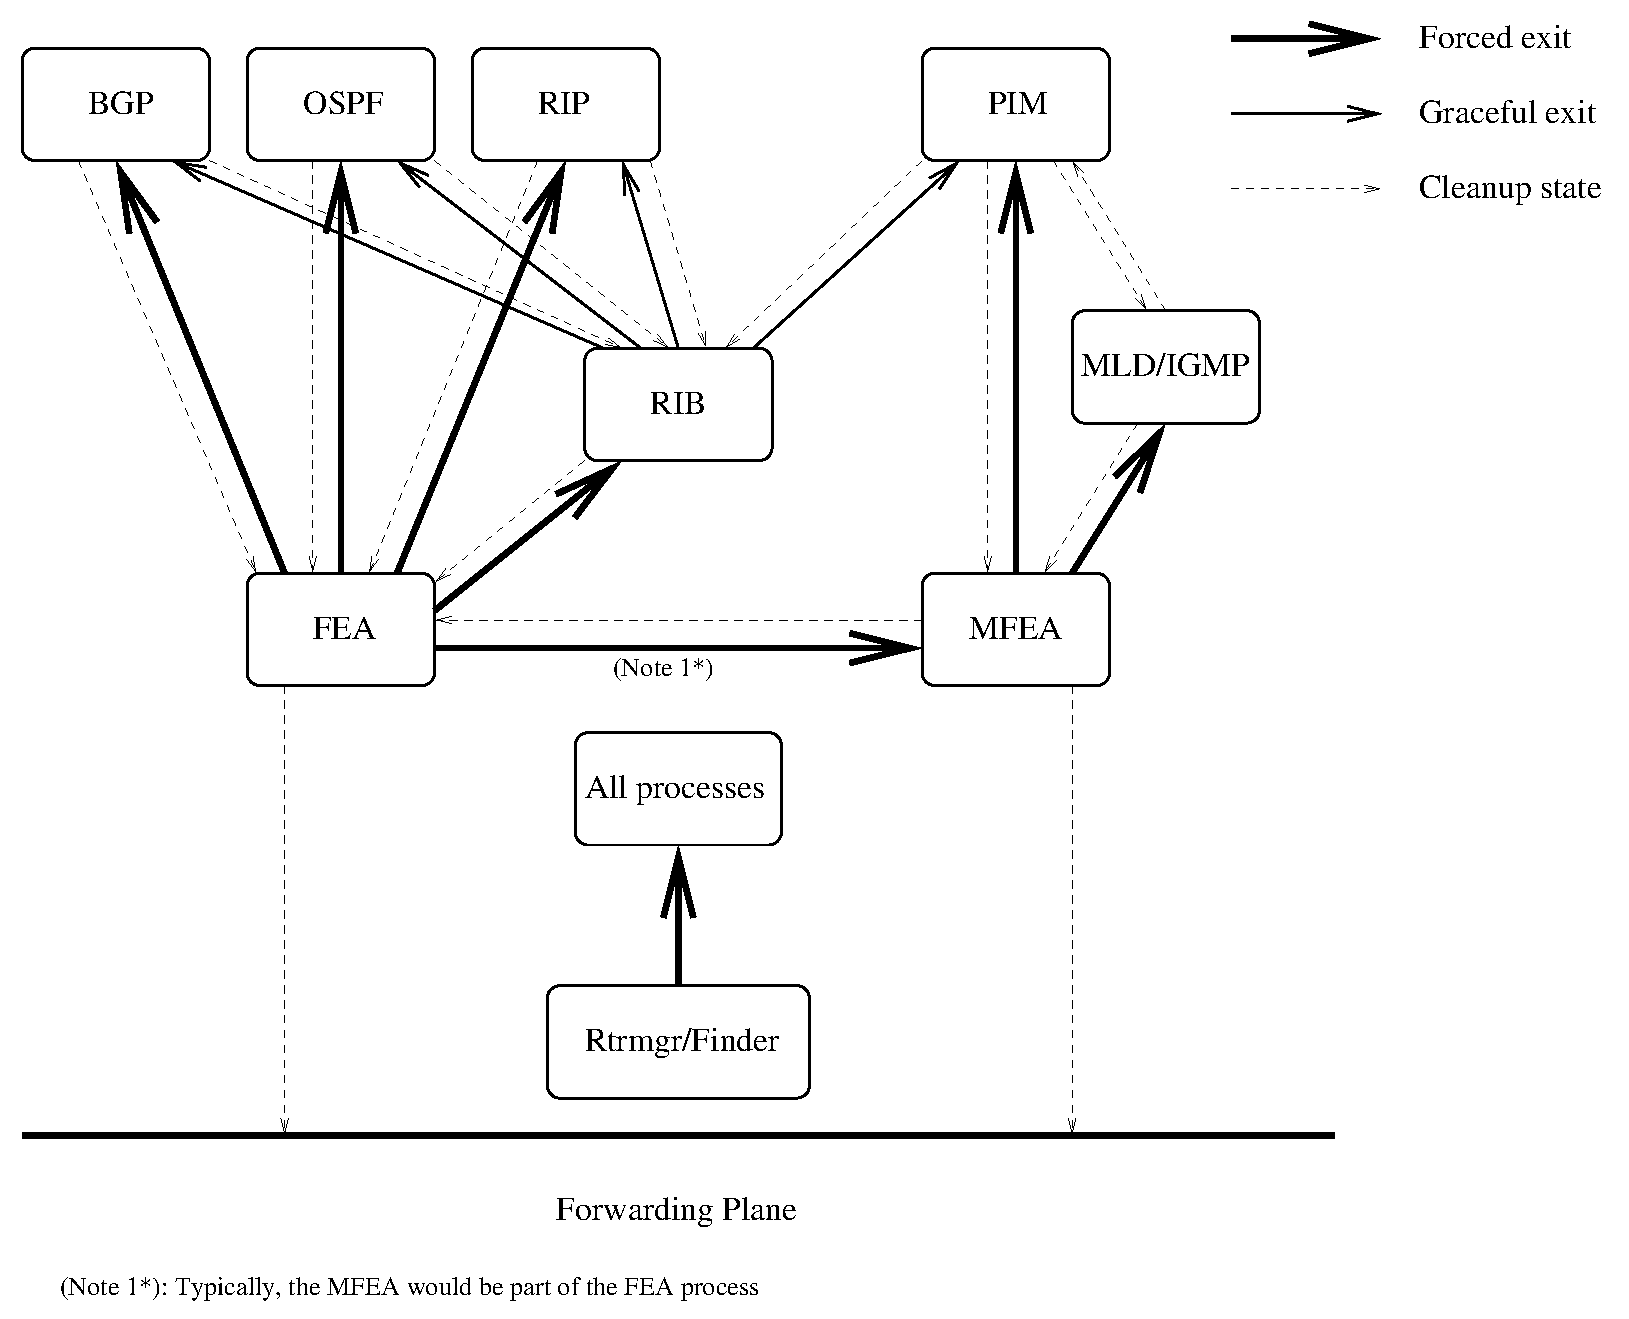
\includegraphics[width=0.9\textwidth]{figs/error_dependency.eps}
    \caption{Process relationship on failure}
    \label{failure_fig}
  \end{center}
\end{figure}

\begin{table}[ht]
\begin{center}
\begin{tabular}{|c|c|c|c|c|c|c|c|c|c|c|}
\hline
Process fails   &                 &          &      &      &      &         &      &      &      &         \\\hline
                & \rtrmgr/        & FEA      & MFEA & RIB  & IGMP & PIM     & BGP  & RIP  & OSPF & \xorpsh \\
                & \finder         &          &      &      &      &         &      &      &      &         \\\hline
\rtrmgr/        & /               & Withdraw & Exit & Exit & Exit & Exit    & Exit & Exit & Exit & Report  \\
\finder         &                 & All      &      &      &      &         &      &      &      & Problem \\
                &                 & Unicast  &      &      &      &         &      &      &      & Wait    \\
                &                 & Routes   &      &      &      &         &      &      &      &         \\
                &                 & Exit     &      &      &      &         &      &      &      &         \\\hline
FEA(*)          &  Restart        & /        & Exit & Exit & Exit & Exit    & Exit & Exit & Exit & -       \\\hline
MFEA(*)         &  Restart        & -        & /    & -    & Exit & Exit    & -    & -    & -    & -       \\\hline
RIB             &  Restart        & Withdraw & /    & -    & Exit & Exit    & Exit & Exit & Exit & -       \\
                &                 & All      &      &      & (G)  & (G)     & (G)  & (G)  & (G)  &         \\
                &                 & Unicast  &      &      &      &         &      &      &      &         \\
                &                 & Routes   &      &      &      &         &      &      &      &         \\\hline
IGMP            &  Restart        & -        & -    & -    & /    & Delete  & -    & -    & -    & -       \\
                &                 &          &      &      &      & Local   &      &      &      &         \\
                &                 &          &      &      &      & Members &      &      &      &         \\
                &                 &          &      &      &      & After   &      &      &      &         \\
                &                 &          &      &      &      & Timeout &      &      &      &         \\\hline
PIM             &  Restart        & -        & -    & -    & -    & /       & -    & -    & -    & -       \\\hline
BGP             &  Restart        & -        & -    & -    & -    & -       & /    & -    & -    & -       \\\hline
BGP             &  Restart        & -        & -    & -    & -    & -       & /    & -    & -    & -       \\\hline
RIP             &  Restart        & -        & -    & -    & -    & -       & -    & /    & -    & -       \\\hline
OSPF            &  Restart        & -        & -    & -    & -    & -       & -    & -    & /    & -       \\\hline
\xorpsh         &  Restart        & -        & -    & -    & -    & -       & -    & -    & -    & /       \\\hline
\end{tabular}
\end{center}
{\small Note(*): Typically, the MFEA would be part of the FEA process}
\caption{\label{failure_table}Action to take on detecting process failure}
\end{table}

%%%%%%%%%%%%%%%%%%%%%%
\subsubsection{\rtrmgr/\finder - Router manager}

If the \rtrmgr/\finder dies then all bets are off and all processes
should exit apart from the \xorpsh.

If a \xorp process exits unexpectedly the \rtrmgr/\finder should
attempt to restart the process.

%%%%%%%%%%%%%%%%%%%%%%
\subsubsection{FEA - Forwarding Engine Abstraction}

The FEA primarily accepts routes from the RIB and places them in the
kernel. The FEA should tag all routes that it has installed in the
kernel.  On restart, the FEA should remove all routes that a previous
incarnation of the FEA has placed in the kernel. When an FEA is
exiting it should attempt to remove all routes that it has installed
in the kernel.

The FEA process should register interest in the RIB. If the RIB fails
the FEA should withdraw all routes that the RIB has sent to it.

%%%%%%%%%%%%%%%%%%%%%%
\subsubsection{MFEA - Multicast Forwarding Engine Abstraction}

The MFEA is multicast analogue to the unicast FEA. If should be noted
that typically the MFEA would be part of the FEA process.

Similar to the FEA, on restart or exit the MFEA should remove all
multicast forwarding entries that were installed in the kernel. Note
that the MFEA does not contain a copy of the multicast forwarding entries
that were installed in the kernel, so it should utilize a
mechanism that removes all multicast forwarding entries at once.  In
case of UNIX-based systems, closing the multicast routing socket will
automatically remove all entries.

If the multicast routing process that has installed the multicast
forwarding entries exits, then the MFEA should remove all multicast
forwarding entries from the kernel. Currently, PIM is the only
multicast routing process. In the future, the XORP multicast routing
architecture may contain a special coordinator among all multicast
routing protocol instances, analogous to the function of the unicast
RIB process. If that coordinator exits, the MFEA should remove all
multicast forwarding entries from the kernel.

%%%%%%%%%%%%%%%%%%%%%%
\subsubsection{RIB - Routing Information Base}

Routes from the routing processes are sent to the RIB; the winners are
sent to the FEA.

The RIB should register interest in the FEA. If the FEA fails the RIB
should exit. All routing processes that interact with the RIB should,
on detecting the shutdown of the RIB, also terminate gracefully.

%%%%%%%%%%%%%%%%%%%%%%
\subsubsection{IGMP/MLD}

If the FEA/MFEA process exits then this process should exit.

%%%%%%%%%%%%%%%%%%%%%%
\subsubsection{PIM}

If the RIB or the FEA/MFEA process exits then this process should exit.

%%%%%%%%%%%%%%%%%%%%%%
\subsubsection{BGP}

Currently the only other process in the system that BGP interacts
with is the RIB. If the BGP process detects that the RIB has died then
it should gracefully terminate its sessions and exit.

In the future the TCP connections that BGP makes will be mediated
through FEA, at which time the BGP process should also register
interest in the state of the FEA. If the BGP process detects the death
of the FEA it should exit immediately.

%%%%%%%%%%%%%%%%%%%%%%
\subsubsection{RIP}

The RIP process should register interest in the FEA and the RIB. If
the RIB dies then the RIP process should attempt to exit gracefully.
If the FEA dies the RIP process should exit immediately.

%%%%%%%%%%%%%%%%%%%%%%
\subsubsection{IS-IS}

The IS-IS process should register interest in the FEA and the RIB. If
the RIB dies then the IS-IS process should attempt to exit gracefully.
If the FEA dies the IS-IS process should exit immediately.

%%%%%%%%%%%%%%%%%%%%%%
\subsubsection{OSPF}

The OSPF process should register interest in the FEA and the RIB. If
the RIB dies then the OSPF process should attempt to exit gracefully.
If the FEA dies the OSPF process should exit immediately.

%%%%%%%%%%%%%%%%%%%%%%
\subsubsection{\label{xorpsh}\xorpsh}

The \xorpsh provides a command line interface to the XORP router.
Other processes in the system exiting should never cause it to
exit. The \rtrmgr/\finder process exiting should generate
warning output to the user and then the \xorpsh should wait for the
router to restart.

%%%%%%%%%%%%%%%%%%%%%%%%%%%%%%%%%%%%%%%%%%%%%%%%%%%%%%%%%%%%%%%%%%%%%%%
\section{XRL Communication Errors}

Interprocess communication in \xorp is achieved using XRLs. In this
section we will consider what should be done when an XRL call fails
due to a communication error.

XRLs can be sent over unreliable transports such as UDP or reliable
transports such as TCP. The type of transport used is decided by the
XRL library based on the specification of each interface.  For the
purposes of error handling, the reliable and unreliable transports are
the same in all regards, except that reliable transports in XORP never
explicitly report a timeout error.

XRL communication is asynchronous: applications request the dispatch
of an XRL and expect to have a callback invoked when the dispatch
result is available.  This presents opportunities for immediate and
deferred error indications.  Immediate error indications occur when
the request for XRL dispatch is made: the canonical example occurring
when no more buffer space is available within the XRL library is
available. An application is able to detect these errors
synchronously: the dispatch request indicates an error in its return
value.  Deferred error indications happen through the dispatch
callbacks.  These callbacks are required to take an XrlError object as
an argument.  An XrlError object is comprised of an enumerated error
code and an optional string containing specific information relating
to the error.  The set of enumerated error codes is presented below.

Immediate and deferred errors are exclusive.  If the \xt dispatching
an XRL got an immediate error, it will not receive a callback
indicating a deferred error.

%%%%%%%%%%%%%%%%%%%%%%%%%%%%%%%%%%%%%%%%%%%
\subsection*{Standard Dispatch XRL Error Values}

The standard XRL return values are returned to the requesting \xt by
the dispatching \xt.  When any of these values are returned, the XRL
communication has been successful.

\begin{description}

  \item [OKAY] XRL dispatch successful.  Additional parameters in
  XRL callback contain return values.

  \item [COMMAND\_FAILED] XRL reached dispatcher, but could not be
  dispatched. The reason for failure may be specified in the note
  associated with the XrlError object.

  \item [BAD\_ARGS] XRL reached dispatcher, but argument types did not match
  those expected by the dispatcher.

\end{description}

%%%%%%%%%%%%%%%%%%%%%%%%%%%%%%%%%%%%%%%%%%%
\subsection*{Finder XRL Error Values}

\begin{description}

  \item [NO\_FINDER] This error occurs when an \xt cannot communicate
  with the \finder. This always indicates a serious problem with the
  router, as the \finder should always be present. The application
  SHOULD treat this error as fatal.

  \item [RESOLVE\_FAILED] This error occurs when a \xt process tries to
  resolve an XRL the \finder has no result for.  This may be because the
  target specified in the XRL does not exist or exists, but is still in
  the process of registering the XRL it exports.

  RESOLVE\_FAILED errors may happen because of a benign cause, namely
  that processes started up in a less than perfect order, so a target's
  user has initialized before the target itself. Applications SHOULD
  handle this type of transient RESOLVE\_FAILED error with a
  retransmission strategy.  Applications may avoid this error by using
  the Finder event observer interface to detect when the particular
  target becomes ready.

  \item [NO\_SUCH\_METHOD] This error occurs when the named \xt is running and
  has registered 
  it's XRLs, but it does not support the method named in the XRL.
  NO\_SUCH\_METHOD generally indicates a version mismatch between two
  processes. This error may be considered fatal, or (for example) the
  application might react by trying to access an older version of the
  interface. The application can expect, however, that NO\_SUCH\_METHOD
  errors are not transient: If an XRL access gets a NO\_SUCH\_METHOD
  error, then that XRL will always result in a NO\_SUCH\_METHOD error,
  at least until the target process restarts.

\end{description}

%%%%%%%%%%%%%%%%%%%%%%%%%%%%%%%%%%%%%%%%%%%
\subsection*{Transport and Internal Xrl Error Values}

\begin{description}

  \item [SEND\_FAILED] The underlying XRL transport mechanism has failed.
  For example, the TCP connection has been reset, or a UDP connection
  gets a port-unreachable message. The expectation is that no further
  communication with the specific endpoint will succeed.

  \item [SEND\_FAILED\_TRANSIENT] This error occurs when the XRL library
  temporarily cannot send a particular XRL. Usually, this will be
  because of congestion or a slow receiver: the kernel has run out of
  buffer space. Note that the XRL library performs some buffering
  itself, to ensure that XRL requests are either completely transmitted
  or not transmitted at all.
  \emph{Note: The XRL library does not yet implement this error.}

  \item [REPLY\_TIMED\_OUT] -- The target did not reply within a
  transport-protocol-specific period of time. Possible reasons include
  network congestion, peer failure, network interface failure, and so
  on. As in all network communications, when a timeout occurs we don't
  know if the last unacknowledged XRL request was received and processed
  by the peer. This error occurs in unreliable transmit only.

\end{description}

%%%%%%%%%%%%%%%%%%%%%%%%%%%%%%%%%%%%%%%%%%%
\subsection{Handling XRL Errors}

XRLs may be directed to a class of target or a particular instance of
a target.  The first instance of a target that registers with the
\finder is considered to be the primary instance of its class and XRLs
addressed to that are directed to that instance.  The XRL library MAY
hide certain REPLY\_TIMED\_OUT and SEND\_FAILED errors for XRLs
directed towards classes, \ie should the instance which is acting as
the primary instance fail or exit, then another instance in that
class, will receive the class directed XRL requests.

%When communication with a particular
%instance of the target fails, the XRL library thus MAY search for
%another instance by contacting the \finder. The XRL library MUST NOT
%perform this retransmission, however, unless it can guarantee that the
%request was not acted on by any instance. (This rules out most
%unreliable transports.) If it cannot guarantee this, or if
%retransmission fails, the XRL will get an error -- either
% REPLY\_TIMED\_OUT, SEND\_FAILED, NO\_FINDER, or RESOLVE\_FAILED.
%
% XXX This is very MIT a la Gabriel's Worse-is-Better :-)  I like it,
% but would rather not commit to this just now
%

The XRL errors of NO\_FINDER, RESOLVE\_FAILED, and to some extent
NO\_SUCH\_METHOD generally represent serious problems with the router.
SEND\_FAILED represents a serious problem with the target, such as
that an instance of the target has died; this problem may or may not
be transient. The SEND\_FAILED\_TRANSIENT and REPLY\_TIMED\_OUT errors
are
potentially common errors, and should be handled by the
application. However, the likelihood of SEND\_FAILED\_TRANSIENT can
often be reduced, making it a ``fatal'' error from the application's
point of view, by limiting the rate at which requests are sent.

NO\_FINDER, RESOLVE\_FAILED, NO\_SUCH\_METHOD, and
SEND\_FAILED\_TRANSIENT, are all indications that the XRL was not
communicated to its target. They are therefore called \emph{send
failures}.  The other two errors, REPLY\_TIMED\_OUT and SEND\_FAILED,
may be generated even if the target received the request. They are
therefore called \emph{receive failures}.

If a peer dies, we will receive notification of this explicitly and
will deal with it as specified in section \ref{pfailure}. Thus most
XRL transport errors SHOULD NOT be taken as an indication that the
peer is definitely dead. If an application cares that the peer has
died or restarted, it SHOULD register with the finder to receive
notifications of process restarts. Thus, a process SHOULD assume that
an XRL transport problem will be transient until it receives an
explicit confirmation that the destination has failed, particularly
when the XRL interface is unreliable.

In addition to an XRL interface being reliable or unreliable, the way
the application uses an XRL interface can by pipelined or
non-pipelined.  In the pipelined case, multiple requests can be
outstanding simultaneously; in the non-pipelined case at most one
request can be outstanding at a time.

It is useful for us to categorize XRL interfaces along these two axes:
reliable/unreliable and pipelined/non-pipelined. 

%%%%%%%%%%%%%%%%%%%%%%%%%%%%%%%%%%%%%%%%%%%
\subsection*{Unreliable, Non-pipelined}

If an XRL send failure occurs, the sending application MAY choose to
retransmit the XRL, or ignore the failure as it sees fit.  

In an XRL receive failure occurs, the sending application MAY also choose
to retransmit the XRL, or ignore the failure as it sees fit. However, if
the application chooses to re-send the XRL, the interface MUST be written
in such a way that the receipt of a duplicate request will not damage the
system. (XXX Isn't this true anyway? Network duplicates?)

%%%%%%%%%%%%%%%%%%%%%%%%%%%%%%%%%%%%%%%%%%%
\subsection*{Reliable, Non-pipelined}

If a SEND\_FAILED\_TRANSIENT error occurs, the sending application MAY
retransmit the XRL.

SEND\_FAILED, NO\_FINDER, and most RESOLVE\_FAILED and
NO\_SUCH\_METHOD errors are unrecoverable.  The application should
cause this XRL interface to go dormant, in the expectation that it
will authoritatively discover from the finder that the target has
died.

REPLY\_TIMED\_OUT cannot happen on reliable interfaces.

%%%%%%%%%%%%%%%%%%%%%%%%%%%%%%%%%%%%%%%%%%%
\subsection*{Unreliable, Pipelined}

The same issues apply as with unreliable, non-pipelined, but the
situation is more complicated.  An interface that uses unreliable
transport and pipelining is one that explicitly permits loss \emph{and
re-ordering} of requests.  It is up to the application to choose
whether to retransmit XRLs that return SEND\_FAILED\_TRANSIENT or
REPLY\_TIMED\_OUT, but the application must only do so if it is
certain that the re-ordering caused by retransmission will not be a
problem.

%%%%%%%%%%%%%%%%%%%%%%%%%%%%%%%%%%%%%%%%%%%
\subsection*{Reliable, Pipelined}

The XRL library ensures that pipelined messages sent to a reliable target
are delivered in order. In particular, if a request $R$ to a given target
gets an error, then no \emph{outstanding} requests to that target
\emph{registered later than $R$} will successfully complete -- they will
all get the same error, and none of them will be delivered to the receiving
application. Once the error is delivered, this error state is wiped out,
and later requests to the target may succeed -- perhaps because the target
was restarted.

Again, SEND\_FAILED, NO\_FINDER, and most RESOLVE\_FAILED and
NO\_SUCH\_METHOD errors are unrecoverable.
The application SHOULD cause this XRL interface to go dormant, in the
expectation that it will authoritatively discover from the finder that
the target has died.

%%%%%%%%%%%%%%%%%%%%%%%%%%%%%%%%%%%%%%%%%%%%%%%%%%%%%%%%%%%%%%%%%%%%%%%
\section{Execution Error}

A XORP router is partitioned into many processes; most of the operating
system specific interactions are performed by the FEA. In a router the
most frequent operation will be the adding and deleting of routes.
Consider BGP adding a route. First the BGP process will send the route
to the RIB, then the route may be sent to the FEA. If the addition of the
route from the RIB to the FEA fails, then there is no way of
propagating this failure back to the BGP process due to the
asynchronous nature of XRLs. If adding/deleting a route fails a very
drastic way of propagating this failure back to the BGP process would
be for either or both the FEA and RIB processes to exit, in which case
the process failure responses already described would be used and BGP
would exit. Process exit is an extreme response to failing
to add a route, but at least the error handling code for process exit
exists already. It is important though not
to mask over implementation problems by ignoring errors. In the rest
of this section we will outline how to deal with a number of common
errors.

%%%%%%%%%%%%%%%%%%%%%%%%%%%%%%%%%%%%%%%%%%%
\subsection{Adding/Deleting route failures}

As stated above, a highly likely error is failures when adding or
deleting routes. Typically the interaction will occur between the RIB
and FEA. When an error occurs it should be logged by the FEA and the
cause returned to the RIB. The RIB can be configured with policy on
how to react to different errors.

Adding a route will typically fail because a route already exists.
Firstly, if a route already exists it is either the same or different
to the one that we attempted to add. Secondly, either the FEA
installed the route or a third party installed it. Therefore when
adding a route fails the FEA should return if the current route is the
same or different to the one we attempted to add, as well as who
installed the route originally. The RIB on receiving the error state
from the FEA can decide as a matter of policy how to proceed. If an
attempt to add a route fails because a different route exists the RIB
could choose to delete the old route and add the new route.

The most common reason for a route deletion to fail would be that the
route is no longer present. The FEA should log that it has been asked
to delete a route that doesn't exist. The RIB should decide if this
problem should be considered fatal.

%%%%%%%%%%%%%%%%%%%%%%
\subsubsection{Route Add Failure due to Resource Starvation}

When a routing process sends a route to the RIB, the asynchronous
nature of XRL handling means that the RIB will typically accept the
route before it has finished processing the addition, and certainly
before it attempts to pass the route to the FEA, and hence on into the
forwarding engine.  It is possible for the route addition to fail due
to memory exhaustion in either the RIB or in the forwarding engine
itself.  Should this occur, it is important for the routing protocol
to be made aware of the event, because the routing information will
now be out of synchronization with the forwarding information.

If the forwarding engine refuses the route due to resource starvation,
the FEA will receive the failure.  The FEA will then indicate
asynchronously to the RIB that the failure occurred.  The RIB will in
turn delete all state from all routing protocols that contributed
versions of this route, and asynchronously pass the failure up to
those routing protocols.  Each of those routing protocols will then
handle the failure in a protocol specific manner.

If the failure occurs due to resource starvation in the RIB, a similar
process will be initiated.  It is not currently clear how to reliably
notify a routing protocol in the case when the router is running out
of memory for user-space processes.

In the case of BGP, if a route fails to be added due to resource
starvation, the simplest mechanism is to take down the peering that
originated the route.  The normal peer reinitialization mechanism
(after some time delay) will ensure that all the routes are
re-instantiated after the resource starvation problem goes away.

In the case of RIP, if a route fails to be added due to resource
starvation, the simplest mechanism is to send our peers an infinite
metric route for this particular prefix and to delete the state for
this prefix.  The normal RIP periodic update will ensure that the
route is re-instantiated after the resource starvation problem goes
away.

In the case of link-state protocols such as OSPF and IS-IS, there is
no good way to deal with this situation.  A reasonable solution might
be to take down all adjacencies to avoid causing a blackhole, then to
bring up the adjacencies again but not propagate any link-state
advertisements to our neighbors (so they won't route via us) until all
the link-state advertisements have been received and we've
successfully installed all the routes in the kernel.

%%%%%%%%%%%%%%%%%%%%%%%%%%%%%%%%%%%%%%%%%%%%%%%%%%%%%%%%%%%%%%%%%%%%%%%
%     APPENDIX
%%%%%%%%%%%%%%%%%%%%%%%%%%%%%%%%%%%%%%%%%%%%%%%%%%%%%%%%%%%%%%%%%%%%%%%
\appendix
\section{Modification History}

\begin{itemize}

  \item June 9, 2003: Initial version 0.3 completed.

  \item August 28, 2003: Updated the version to 0.4, and the date.

  \item November 6, 2003: Updated the version to 0.5, and the date.

  \item July 8, 2004: Updated the version to 1.0, and the date.

  \item April 13, 2005: Updated the version to 1.1, and the date.

  \item March 8, 2006: Added a footnote about the policy manager process.
  Updated the version to 1.2, and the date.

  \item August 2, 2006: Added ``Modification History'' appendix.
  Updated the version to 1.3, and the date.

  \item March 20, 2007: Updated the version to 1.4, and the date.

\end{itemize}

%%%%%%%%%%%%%%%%%%%%%%%%%%%%%%%%%%%%%%%%%%%%%%%%%%%%%%%%%%%%%%%%%%%%%%%
%     BIBLIOGRAPHY
%%%%%%%%%%%%%%%%%%%%%%%%%%%%%%%%%%%%%%%%%%%%%%%%%%%%%%%%%%%%%%%%%%%%%%%
\bibliography{../tex/xorp}
\bibliographystyle{plain}

%%%%%%%%%%%%%%%%%%%%%%%%%%%%%%%%%%%%%%%%%%%%%%%%%%%%%%%%%%%%%%%%%%%%%%%
\end{document}
